% Author: Izaak Neutelings (October 2020)
% Inspiration: https://tex.stackexchange.com/questions/25531/adding-underbrace-in-tikz
\documentclass[border=3pt,tikz]{standalone}
\usepackage{physics}
\usepackage{siunitx}
\usepackage{ifthen}
\usepackage{tikz}
\usepackage[outline]{contour} % glow around text
\usetikzlibrary{calc}
\usetikzlibrary{angles,quotes} % for pic
\usetikzlibrary{patterns,snakes}
\tikzset{>=latex} % for LaTeX arrow head
\contourlength{1.4pt}

\colorlet{xcol}{blue!70!black}
\colorlet{vcol}{green!60!black}
\colorlet{myred}{red!65!black}
\colorlet{acol}{red!50!blue!80!black!80}
\tikzstyle{mass}=[line width=0.6,red!30!black,fill=red!40!black!10,rounded corners=1,
                  top color=red!40!black!20,bottom color=red!40!black!10,shading angle=20]
\tikzstyle{faded mass}=[dashed,line width=0.1,red!30!black!40,fill=red!40!black!10,rounded corners=1,
                        top color=red!40!black!10,bottom color=red!40!black!10,shading angle=20]
\tikzstyle{rope}=[brown!70!black,very thick,line cap=round]
\def\rope#1{ \draw[black,line width=1.4] #1; \draw[rope,line width=1.1] #1; }
\tikzstyle{force}=[->,myred,very thick,line cap=round]
\tikzstyle{velocity}=[->,vcol,very thick,line cap=round]
\tikzstyle{Fproj}=[force,myred!40]

\begin{document}


% SKI RAMP
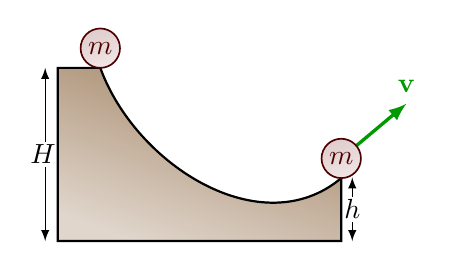
\begin{tikzpicture}
  \def\H{2.2} % height start
  \def\h{0.8} % height final
  \def\L{3.6} % length
  \def\R{0.25} % ball radius
  \coordinate (L) at (0,\H);
  \coordinate (A) at (0.15*\L,\H);
  \coordinate (B) at (\L,\h);
  \draw[<->] (-0.16,0) --++ (0,\H) node[midway,left=-5,fill=white,inner sep=1] {$H$};
  \draw[<->] (\L+0.14,0) --++ (0,\h+0.01) node[midway,fill=white,inner sep=1] {$h$};
  \draw[thick,top color=orange!40!black!60,bottom color=orange!40!black!20,shading angle=-20]
    (L) -- (A) to[out=-70,in=-140] (B) |- (0,0) -- cycle; %,line cap=round
  %\draw[force] (M)++(140:0.7*\r) --++ (-\F,0) node[below=1,above left=-4] {$\vb{F}_\mathrm{c}$};
  \draw[force,vcol] (B)++(0,\R) --++ (40:0.3*\L) node[above=0] {$\vb{v}$};
  \draw[thin,mass] (A)++(0,\R) circle(\R) node[] {$m$};
  \draw[thin,mass] (B)++(0,\R) circle(\R) node[] {$m$};
\end{tikzpicture}


% PENDULUM UP
\def\L{2.8} % length
\def\ang{32} % length
\def\R{0.25} % ball radius
\begin{tikzpicture}
  \coordinate (M) at (\ang-90:\L);
  \coordinate (M') at (0,-\L);
  \coordinate (O) at (0,0);
  \coordinate (B) at (0,-\L-1.4*\R);
  \draw[faded mass] (M') circle(\R);
  \draw[dashed] (O) -- (B);
  \draw[dashed] (M')++(-0.7*\R,0) --++ ({0.65*\L*sin(\ang)},0) coordinate (A);
  \draw[dashed] (M')++(-0.7*\R,{\L-\L*cos(\ang)}) --++ ({1.2*\L*sin(\ang)},0);
  \draw[<->] (A)++(-0.2*\R,0) --++ (0,{\L-\L*cos(\ang)}) node[midway,right=-1] {$h$};
  \rope{(O) -- (M)} \path (O) -- (M) node[midway,right=1] {$L$};
  \fill[black] (O) circle(0.04);
  %\draw[force] (M)++(140:0.7*\r) --++ (-\F,0) node[below=1,above left=-4] {$\vb{F}_\mathrm{c}$};
  \draw[mass] (M) circle(\R) node {$m$};
  \draw pic[->,"\,$\theta_\text{max}$",xcol,draw=xcol,angle radius=29,angle eccentricity=1.3] {angle=B--O--M};
\end{tikzpicture}


% PENDULUM 
\begin{tikzpicture}
  \coordinate (M) at (0,-\L);
  \coordinate (O) at (0,0);
  \rope{(O) -- (M)} \path (O) -- (M) node[midway,right] {$L$};
  \fill[black] (O) circle(0.04);
  \draw[velocity] (M)++(-\R,0) --++ (-2.7*\R,0) node[above=0] {$\vb{v}$};
  \draw[mass] (M) circle(\R) node {$m$};
\end{tikzpicture}


% BALLISTIC PENDULUM before
\def\L{2.8} % length
\def\w{0.8} % box width
\def\h{0.5} % box height
\begin{tikzpicture}
  \coordinate (M) at (0,-\L);
  \coordinate (O) at (0,0);
  \coordinate (B) at (-3*\w,-\L);
  \rope{(O) -- (M)} \path (O) -- (M) node[midway,right] {$L$};
  \fill[black] (O) circle(0.04);
  \draw[mass] (M)++(-\w/2,-\h/2) rectangle++ (\w,\h) node[midway] {$M$};
  \draw[velocity] (B) --++ (1.9*\w,0) node[above=0] {$\vb{v}$};
  \draw[very thin,fill=black!60]
    (B)++(-0.06,0.05) --++ (0.06,0) arc(90:-90:0.08 and 0.05) -| cycle
    node[midway,below=2] {$m$};
\end{tikzpicture}


% BALLISTIC PENDULUM hit
\def\L{2.8} % length
\def\w{0.8} % box width
\def\h{0.5} % box height
\begin{tikzpicture}
  \coordinate (M) at (0,-\L);
  \coordinate (O) at (0,0);
  \coordinate (B) at (-0.35*\w,-\L);
  \rope{(O) -- (M)} \path (O) -- (M) node[midway,right] {$L$};
  \fill[black] (O) circle(0.04);
  \draw[velocity] (M)++(\w/2,0) --++ (0.6*\w,0) node[above=0] {$\vb{v}'$};
  \draw[mass] (M)++(-\w/2,-\h/2) rectangle++ (\w,\h);
  \draw[very thin,fill=black!60]
    (B)++(-0.06,0.05) --++ (0.06,0) arc(90:-90:0.08 and 0.05) -| cycle;
\end{tikzpicture}


% BALLISTIC PENDULUM up
\def\L{2.8}  % length
\def\w{0.8}  % box width
\def\h{0.5}  % box height
\def\ang{30} % angle
\begin{tikzpicture}
  \coordinate (M') at (0,-\L);
  \coordinate (M) at (\ang-90:\L);
  \coordinate (O) at (0,0);
  \coordinate (B) at ({\L*sin(\ang)-0.35*\w*cos(\ang)},{-\L*cos(\ang)-0.35*\w*sin(\ang)});
  \draw[faded mass] (M')++(-\w/2,-\h/2) rectangle++ (\w,\h);
  \draw[dashed] (O) -- (M');
  \draw[dashed] (M')++(-0.2*\w,0) --++ ({0.6*\L*sin(\ang)},0) coordinate (A);
  \draw[dashed] (M')++(-0.2*\w,{\L-\L*cos(\ang)}) --++ ({1.1*\L*sin(\ang)},0);
  \draw[<->] (A)++(-0.2*\w,0) --++ (0,{\L-\L*cos(\ang)}) node[midway,right=-1] {$h$};
  \rope{(O) -- (M)} \path (O) -- (M) node[midway,right] {$L$};
  \fill[black] (O) circle(0.04);
  \draw[mass,rotate=\ang] (M)++(-\w/2,-\h/2) rectangle++ (\w,\h);
  \draw[very thin,fill=black!60,rotate=\ang]
    (B)++(-0.06,0.05) --++ (0.06,0) arc(90:-90:0.08 and 0.05) -| cycle;
  \draw pic[->,"\,$\theta_\text{max}$",xcol,draw=xcol,angle radius=29,angle eccentricity=1.3] {angle=M'--O--M};
\end{tikzpicture}


\end{document}